\documentclass{beamer}

%%%%%%%%%%%%
% PACKAGES %
\usepackage{amsmath}
\usepackage{color}

%%%%%%%%%
% THEME %
\usetheme{Warsaw}
\setbeamertemplate{navigation symbols}{}

%%%%%%%%%%%%%%%%%%%
% CUSTOM COMMANDS %
\DeclareMathOperator{\Tr}{Tr}
	\DeclareMathOperator*{\Cov}{Cov}
	\DeclareMathOperator{\cov}{Cov}

	\newcommand{\ket}[1]{\ensuremath{\vert #1 \rangle}}
	\newcommand{\bra}[1]{\ensuremath{\langle #1 \vert}}
	\newcommand{\braket}[2]{\ensuremath{\langle #1 \vert #2 \rangle}}
	\newcommand{\braOket}[3]{\ensuremath{\langle #1 \vert #2 \vert #3 \rangle}}
	\newcommand{\ketbra}[2]{\ensuremath{\vert #1 \rangle \! \langle #2 \vert}}
	\newcommand{\expect}[1]{\ensuremath{\langle #1 \rangle}}
	\newcommand{\varian}[1]{\ensuremath{\left(\Delta #1 \right)^2}}
	\newcommand{\ver}[2]{\ensuremath{\genfrac{}{}{0pt}{}{#1}{#2}}}
	\newcommand{\tr}[1]{\ensuremath{\Tr \lcua #1\rcua}}
	\newcommand{\trsub}[2]{\ensuremath{\Tr_{#1} \lcua #2 \rcua }}
	\newcommand{\bsym}[1]{\ensuremath{\boldsymbol{#1}}}
	\newcommand{\citate}[1]{\footnotesize{\color{gray}[ #1 ]}

	}

	\def\be{\begin{equation}}
	\def\ee{\end{equation}}
	\def\bea{\begin{eqnarray}}
	\def\eea{\end{eqnarray}}
	\def\bse{\begin{subequations}}
	\def\ese{\end{subequations}}
	\def\mtxid{\mathbbm{1}}
	\def\lpar{\left(}
	\def\rpar{\right)}
	\def\lcua{\left[}
	\def\rcua{\right]}
	\def\lcor{\left\{}
	\def\rcor{\right\}}
	\def\lang{\left\langle}
	\def\rang{\right\rangle}
	\def\l{\left}
	\def\r{\right}
	\def\nnnl{\nonumber\\}
	\def\nnnlq{\nonumber\\ && \quad}
	\def\nnnlqq{\nonumber\\ && \qquad}
	\def\nnnlqqq{\nonumber\\ && \quad\qquad}
	\def\ie{, \textit{i.e.}, }
	\def\etal{\textit{et al. }}

%%%%%%%%%%%%%%%%
% THE DOCUMENT %
\begin{document}

%%%%%%%%%%%%%%
% TITLE PAGE %
\title{Optimal bound on the quantum\\ Fisher Information}

	\subtitle{\it Based on few initial expectation values of the prove state.
	}

	\author[Iagoba, Matthias, Otfried, G\'eza]{
		{\bf Iagoba Apellaniz} \inst{1},
		Matthias Kleinmann \inst{1},
		Otfried Gh\"une \inst{2},
		\& G\'eza T\'oth \inst{1,3,4}
	}
	\institute{
		{\bf iagoba.apellaniz@gmail.com}\\
		\vspace{5px}
		\inst{1}
		Department of Theoretical Physics, University of the Basque Country, Spain\\
		\inst{2}
		Naturwissenschaftlich-Technische Fakult\"at, Universit\"at Siegen, Germany\\
		\inst{3}
		IKERBASQUE, Basque Foundation for Science, Spain\\
		\inst{4}
		Wigner Research Centre for Physics, Hungarian Academy of Sciences, Hungary
	}


	\date{Recent Advances in Quantum Metrology; Warsaw - 2016}


%%%%%%%%%%%%%%%%
% BEGIN FRAMES %
\begin{frame}
	\titlepage
\end{frame}

% Reset counter to skip title page
\addtocounter{framenumber}{-1}
	\addtobeamertemplate{navigation symbols}{}{%
    \usebeamerfont{footline}%
    \usebeamercolor[fg]{footline}%
    \hspace{1em}%
    \insertframenumber/\inserttotalframenumber
	}

\begin{frame}
	\frametitle{Outline}
	\tableofcontents
\end{frame}

\section{Introduction and Motivation}

	\begin{frame}
		\begin{enumerate}
			\item<1-> \emph{\color{blue} Many \bf inequalities} have been proposed to lower bound the quantum Fisher Information.
		  	\only<1>{
					\begin{block}{Bounds for qFI}
							\small
							\[\mathcal{F}[\varrho,J_z]\geq 	\frac{\expect{J_x}^2}{\varian{J_y}},
								\qquad\quad
								\mathcal{F}[\varrho,J_y]\geq \beta^{-2}\frac{\expect{J_x^2+J_z^2}}{\varian{J_z}+\frac{1}{4}},
							\]
							\[\mathcal{F}[\varrho,J_z]\geq \frac{4(\expect{J_x^2+J_y^2})^2} {2\sqrt{\varian{J_x^2}\varian{J_y^2}} +\expect{J_x^2} -2\expect{J_y^2}(1+\expect{J_x^2}) +6 }
							\]
					\end{block}
					\citate{\textbf{I.A.}, B. L\"ucke, J. Peise, C. Klempt \& G. Toth, New J. Phys. {\bf 17}, 083027 (2015)}
					\citate{L. Pezz\'e \& A. Smerzi, Phys. Rev. Lett. {\bf 102}, 100401 (2009)}
					\citate{Z. Zhang \& L.-M. Duan, 2014 New J. Phys. {\bf 16} 103037 (2014)}
				}
			\only<2->{
			\item Typically, we only have \emph{\color{blue} a couple of expectation values} to characterize the state.
				\only<2,3>{\begin{figure}
  				\includegraphics<2>[height=120px]{img/ghz3-histogram.pdf}
					\includegraphics<3>[height=120px]{img/ghz3-histogram-banned.pdf}
				\end{figure}}
			}
			\only<4->{
			\item<4->	The archetypical criteria that demonstrates \emph{\color{blue} useful entanglement} on the state.
				\only<4>{
					\[\mathcal{F}[\varrho,J_z]\geq 	\frac{\expect{J_x}}{\varian{J_z}}\]
					\citate{L. Pezz\'e \& A. Smerzi, Phys. Rev. Lett. {\bf 102}, 100401 (2009)}
				}
			}
			\only<5>{
			\item It is essential either to \emph{\color{blue} verify them or find new ones} for different set of expectation values.
			}
		\end{enumerate}

	\end{frame}

\section[QFI based on expectation values]{QFI based on expectation values: Are they optimal?}

	\begin{frame}
		\tableofcontents[currentsection]

	\end{frame}

	\begin{frame}
		\frametitle{The non-trivial exercise of computing the qFI}

		\begin{enumerate}
			\item<1-> Different forms of the qFI
				\begin{block}
					{}
					\small
					\[
						\mathcal{F}[\varrho,J_z]=2 \sum_{\lambda,\gamma} \frac{(p_\lambda-p_\gamma)^2}{p_\lambda+p_\gamma} |\braOket{\lambda}{J_z}{\gamma}|^2
					\]
					\[
					  \mathcal{F}[\varrho,J_z]=\min_{\{p_k,\ket{\Psi_k}\}} 4\sum_k p_k \varian{J_z}_{\ket{\Psi_k}}
					\]
				\end{block}

			\item<2-> For pure states it's extremely simple
				{\small
				\[
					\mathcal{F}[\varrho,J_z] = 4\varian{J_z}
				\]
				}
			\item<3-> In the general case, usually \emph{\color{blue} lower bounded} by its \emph{"classical"} counterparts.

		\end{enumerate}

	\end{frame}

	\subsection{Optimization problem}

		\begin{frame}
			\frametitle{Optimization: Legendre Transform}
			\begin{itemize}
				\item For a convex function of the state, we construct a \emph{thight lower bound} as follows,
					{\small \[
					g(\varrho) \geq
					\mathcal{B} \big( \{w_k := \expect{W_k}\} \big) = \sup_{\{r_k\}} \big( r \cdot w - \sup_{\varrho} [ r\cdot\expect{W} - g(\varrho) ] \big).
					\]}
				\item When $g(\varrho)$ is deffined as infimum over the convex roof, the $2^{\rm nd}$ optimization simplified to pure states only,
					\begin{block}
						{}
						{\small
						\vspace{8px}
						\[
						\mathcal{B}(\{w_k\}) = \sup_{\{r_k\}} \big( r\cdot w - \sup_{\ket{\psi}} [ r\cdot\expect{W} - g(\ket{\psi}) ] \big).
						\]}
					\end{block}
			\end{itemize}

			\citate{O. G\"uhne, M. Reimpell, and R.F. Werner, Phys. Rev.
Lett. {\bf 98}, 110502 (2007)}

		\end{frame}

		\begin{frame}
			\begin{block}
				{Optimization for the qFI}
				Different because of \emph{\color{blue} simplicity of the qFI for pure states}.
				{\small
				\[
				\mathcal{F}(\{w_k\}) = \sup_{\{r_k\}} \big( r\cdot w - \sup_{\mu} [ \lambda_{\max} ( r\cdot W - 4(J_z-\mu)^2 ) ] \big).
				\]}
			\end{block}
			\begin{itemize}
				\item Therefore, we have parametrised the optimization, which leads to a \emph{more efficient finding} of the solution.

			\end{itemize}

			\citate{{\bf I.A.}, M. Kleinmann, O. G\"une \& G. T\'oth, arXiv:1511.05203}

		\end{frame}

\section{Case study}

		\begin{frame}
			\tableofcontents[currentsection]

		\end{frame}

		\begin{frame}
			\begin{itemize}
				\item We'll present 2 main cases, spin-squeezed states and unpolarized Dicke.
				\item Though, we apply our method to projectors with great success, we will focus on global $J_{\mathbf n}$ momentums.
				\item One of the cases using projector operators, {\it i.e.}, using the \emph{fidelity} leads to \emph{\color{blue}analytic soulution}!
			\end{itemize}
			% \onslide{
			\begin{figure}
				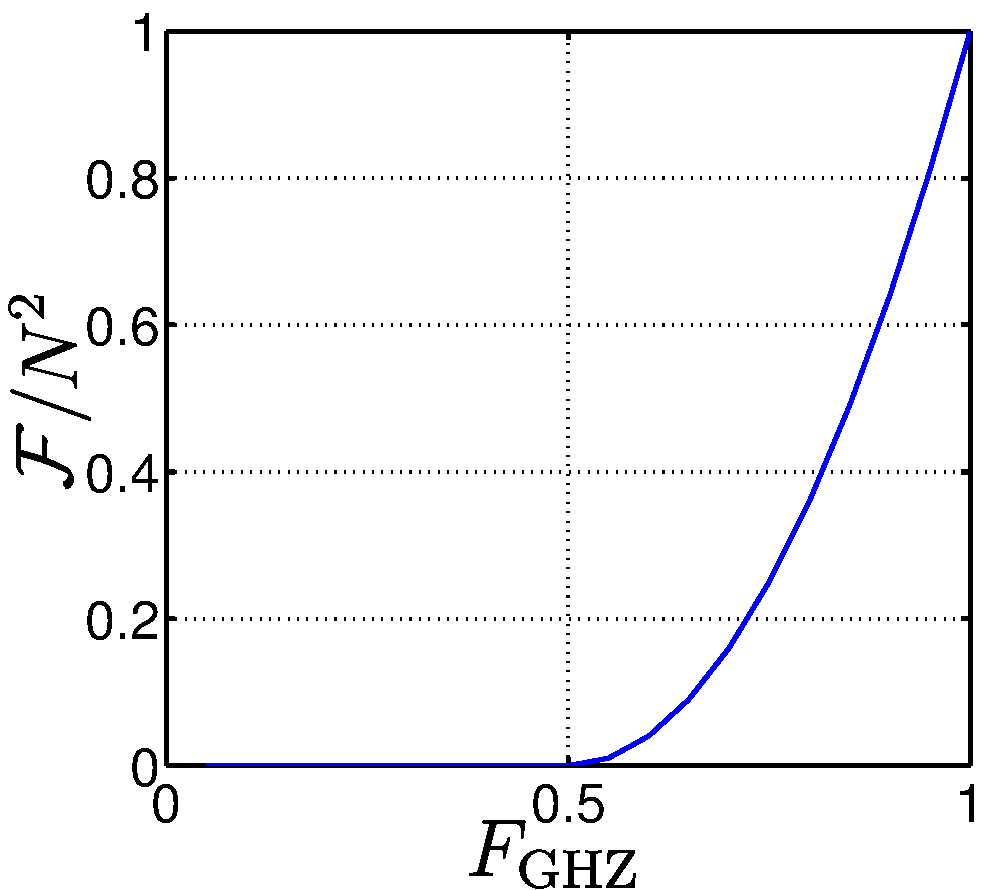
\includegraphics[height=90px]{img/lb-ghzfidelity.pdf}
				\hspace{20px}
				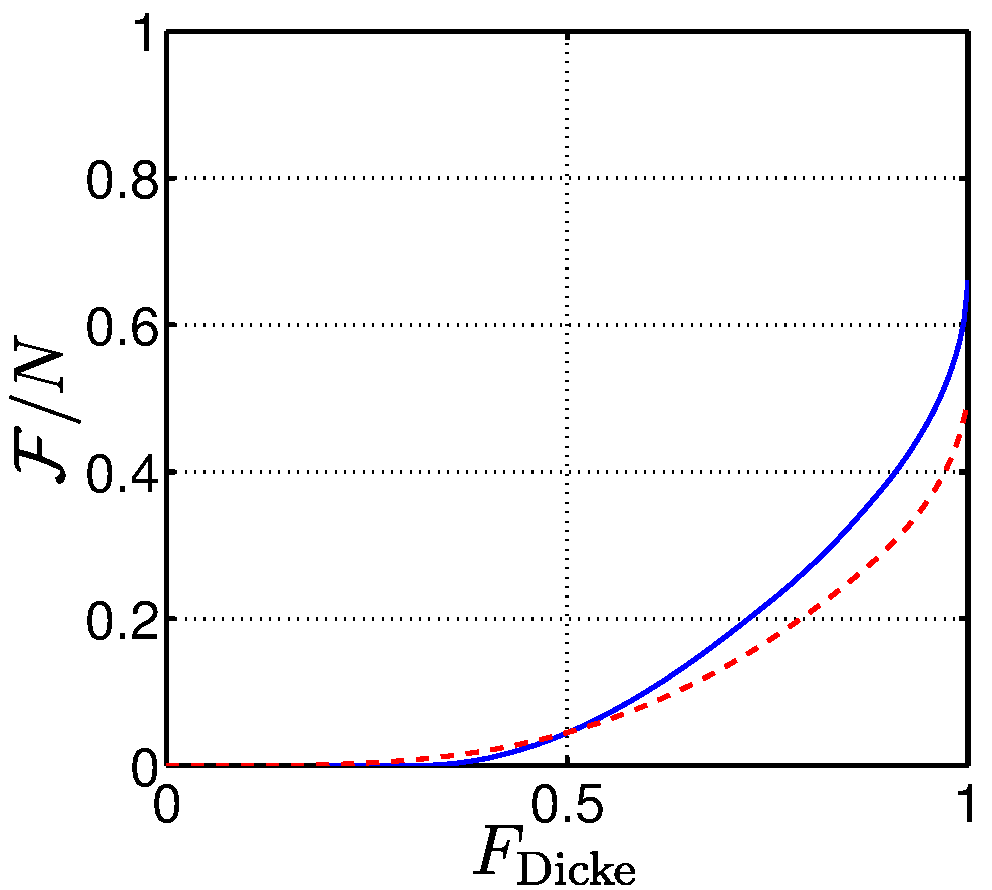
\includegraphics[height=90px]{img/lb-dickefidelity}
			\end{figure}
			% }

		\end{frame}

	\subsection{Spin squeezed states}

		\begin{frame}
			{Measuring $\expect{J_z}$ and $\varian{J_x}$ for Spin Squeezed States}

			\begin{enumerate}
				\item We use the following 3 operators $\{ J_z,J_x,J_x^2 \}$ to characterize the input state with their respective expectation values.
				\item In the direction of $\expect{J_x}$ the worst case is when it takes the \emph{\color{blue}value zero}.
				\item Therefore, the optimisation can be accomplished only for 2 operators $\{ J_z,J_x^2 \}$ while it is mapped directly to $\expect{J_z},\varian{J_x}$.

			\end{enumerate}

		\end{frame}

		\begin{frame}
			\begin{itemize}
				\item We numerically optimise the lower bound of qFI for a 4 particle system for all possible values of $\expect{J_z}$ and $\varian{J_x}$.
			\end{itemize}
			\begin{figure}
				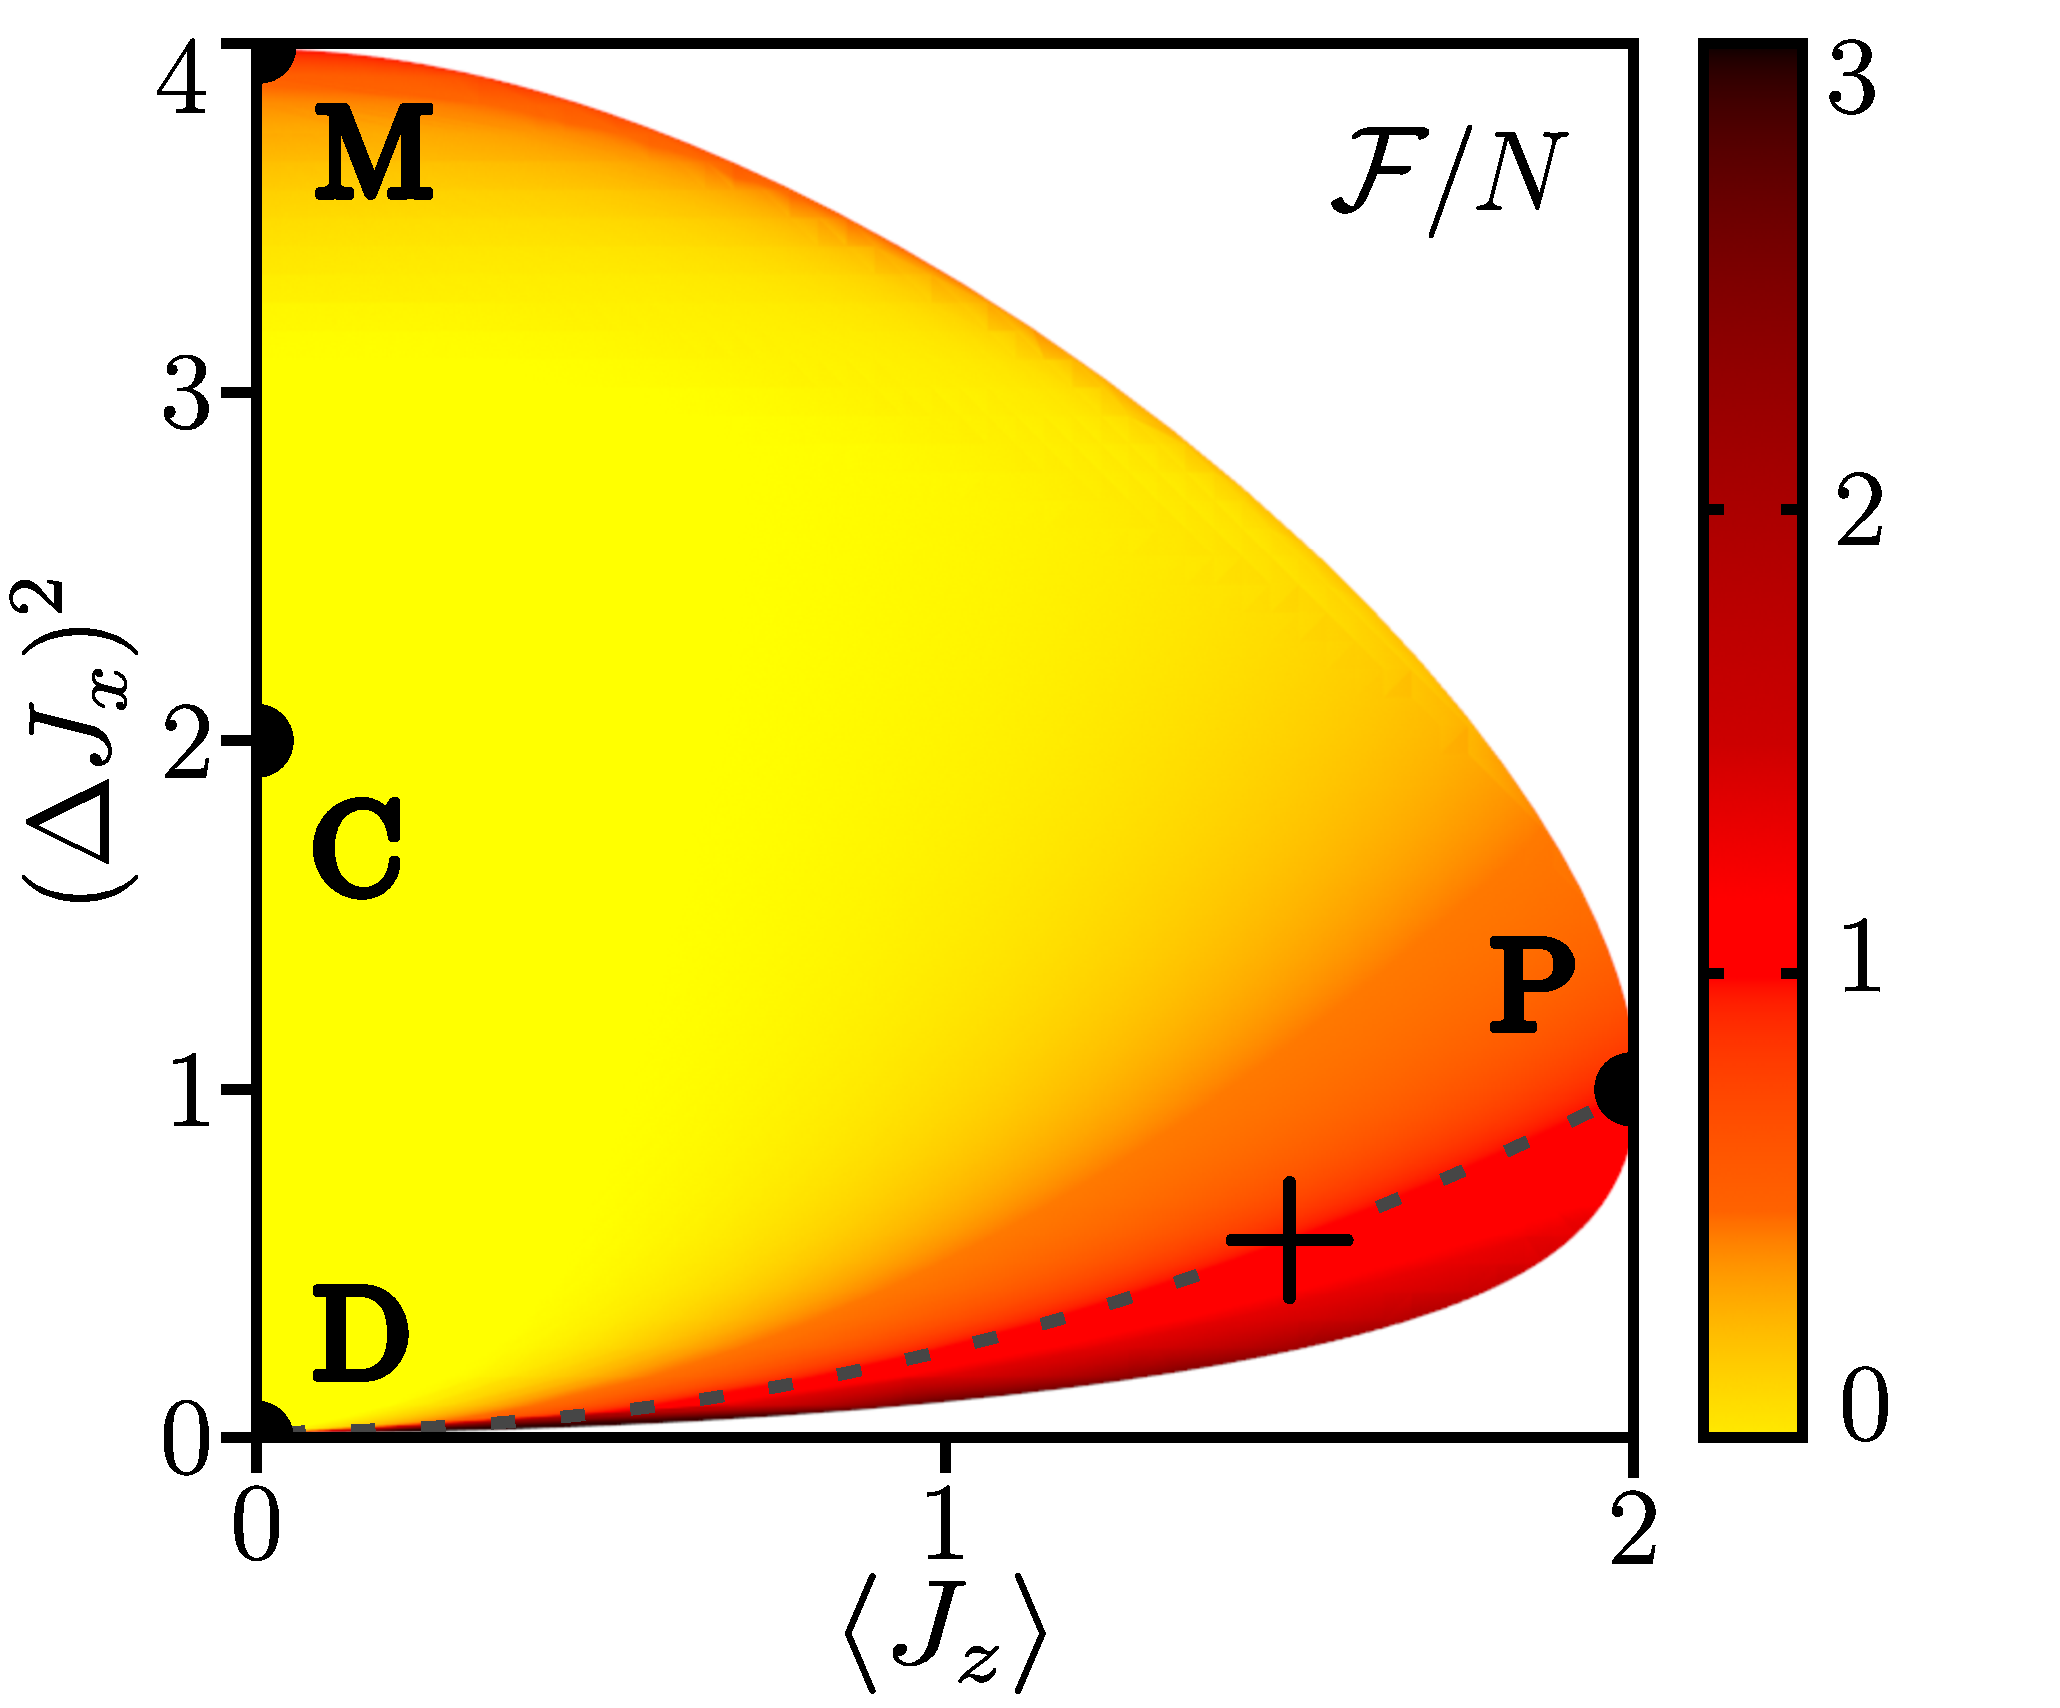
\includegraphics[height=120px]{img/lb-spsq.pdf}
				\caption{Below the dashed line, $\mathcal{F}$ surpasses the shot noise limit. The crossed point to be extended next. It shows an extremely similarity with $\mathcal{F}\geq \expect{J_z}^2/\varian{J_x}$, TODO}
			\end{figure}

		\end{frame}

		\begin{frame}
			\begin{itemize}
				\item For the crossed point, we now study what happens with the extra information of a $3^{\rm rd}$ expectation value.
			\end{itemize}
			\begin{figure}
				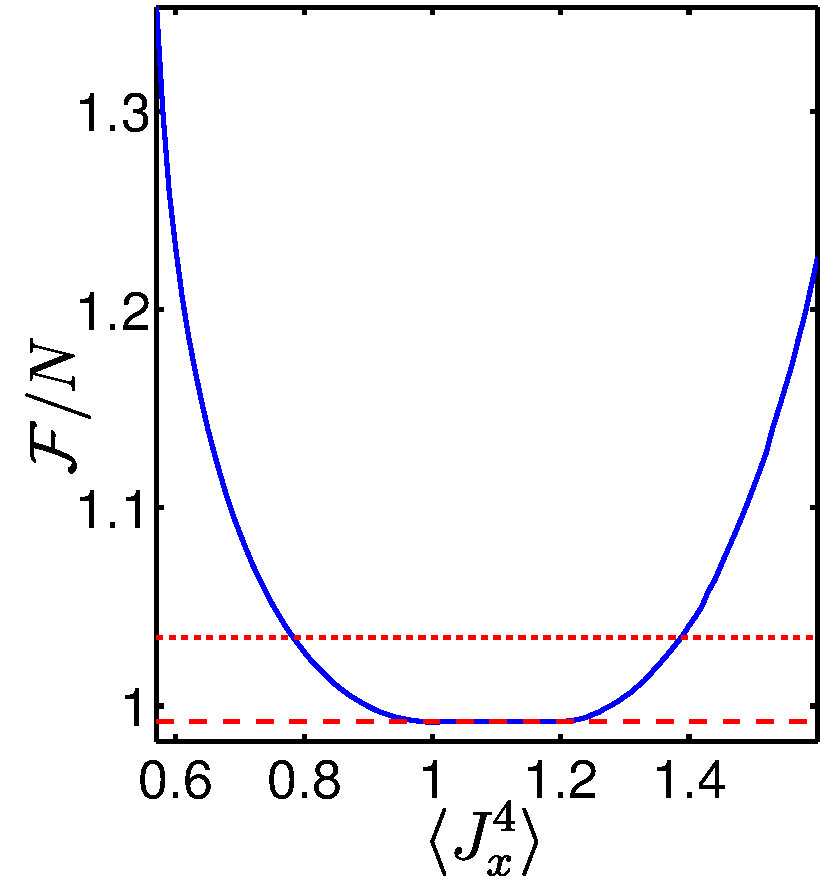
\includegraphics[height=120px]{img/4thparameter-spsq.pdf}
			\end{figure}

		\end{frame}

	\subsection{Unpolarized Dicke states}

		\begin{frame}


		\end{frame}

\section{Conclusion and outlook}

	\begin{frame}
		\frametitle{Conclusion and Outlook}
		\begin{enumerate}
			\item<1-> We have found that on very interesting cases the optimization case is feasible.
			\item<2-> We used our approach to verify the tight bounding of one of the inequalities.
			\item<3-> We have shown that the lower bound can be improved with few extra considerations.
			\item<4-> It has been show that
		\end{enumerate}

	\end{frame}

	\begin{frame}
		\emph{\Large Thank you for your attention!}

		\vspace{5px}
		Group's home page $\rightarrow$ \emph{\color{blue} https://sites.google.com/site/gedentqopt}

	\end{frame}

\end{document}
